\chapter{Design and Implementation}
\label{chapter:design}

Based on the requirements identified in the previous chapter, we're in this chapter introducing the design and implementation details of the of our proposed proxy solution. We get started by discussing the overall design, before we dive into the implementations details.

\section{Overall Design}

In previous chapters we have argued that all optimization techniques should be
placed in proxies in order to retains interoperability for COTS applications,
as well as to break their end-to-end dependency. Our overall design therefore
deploying a proxy pair to facilitate Web communication. The idea is to deploy
the proxy pair in two different locations separated by a DIL network. Through
the locally deployed proxy can then Web applications proxy all their
communication. The proxy will then apply different optimization
techniques, and over over a DIL network forward the request to the other proxy, and
finally return a response. Ideally should a proxy be deployed as close to its
intended user applications as possible, preferable at the same machine.


It is worth noting that since the proxies is designed to accept \textit{all} HTTP
requests, they can support any applications that utilize HTTP, including request-
response and publish-subscribe applications.

\section{Design of Solution}

\subsection{Design of HTTP proxy}

A deployed proxy is designed to accept arbitrary HTTP requests, possible from
multiple clients, and forward them to the other proxy as seen in
\cref{figure:proxy_design}. Ideally the proxy should be deployed as close to its
intended users as possible, as the communication between an application and its
proxy is not subject to any optimization for DIL environments.

\begin{figure}[h]
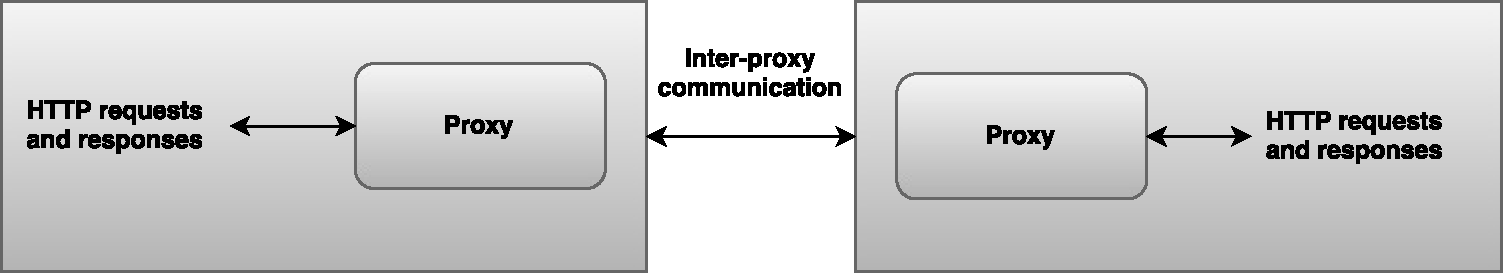
\includegraphics[scale=0.55]{images/proxy_design.pdf}
\caption{Design of Solution}
\label{figure:proxy_design}
\end{figure}

It is the communication between a proxy pair that is subject to optimizations.
The proxies are therefore designed to support the optimization techniques we
have identified. Those are primarily concerned about using different transport
protocols as the inter-proxy communication, as illustrated in
\cref{figure:proxy-communication}. The purpose of this is to evaluate the
performance of the transport protocols in DIL networks. Which protocol to use as
the means of inter-proxy communication is therefore designed to be easily
configured by the user of the proxy.

\begin{figure}[h]
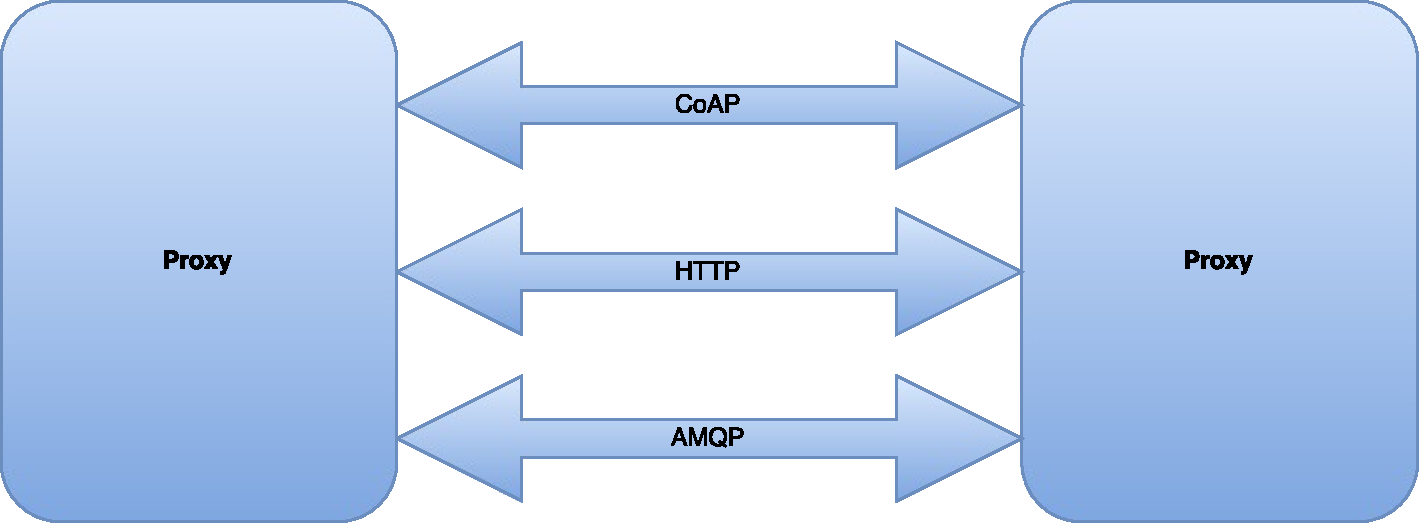
\includegraphics[scale=0.5]{images/proxy_communcation.pdf}
\caption{The proxies were designed to support multiple protocols for inter-proxy communication}
\label{figure:proxy-communication}
\end{figure}

\section{Choosing a framework}

Requirement one implies creating a HTTP proxy which accepts HTTP requests,
forward them, and finally return a HTTP response. We identified some approaches:

\begin{enumerate}
    \item Build a HTTP proxy from scratch ourself.
    \item Use an existing HTTP proxy.
\end{enumerate}

Building a HTTP proxy ourself would allow us to customize our solutions as we
wanted, but would require a lot of implementation. We therefore concluded that
best use of our resources was to use an existing configurable proxy. Building
on state-of-art existing solutions allowing us to focus on the optimization
techniques, rather than on the specific low-level details of HTTP. After some research we found three possible HTTP-proxies:

\begin{enumerate}
    \item Squid
    \item Nginx.
    \item Apache Camel
\end{enumerate}

Apache Camel is an open source Java framework developed by the Apache Software
Foundation for rule-based routing and mediation\cite{camel-homepage}. It has a
wide range of use-cases and focuses on making integration between different
enterprise communication system easier. It support a large set of different
communication transports (transport protocols). We chose to use Apache Camel as
our HTTP proxy due to its simplicity and support for different transport
protocols.

\subsection{Apache Camel}

Routing is a central concept in Apache Camel and consist of defining a
\textit{from route}. This is an endpoint from which Camel consumes messages. It
can then invoke a series of \textit{processors}, which can modify the headers,
payload etc. of the message. Then, Camel forwards the message to a \textit{to
route}, which can be an application running somewhere else. When a response is
received, Camel can invoke a new set of processors on the message, before it is
finally returned to the origin. An overview of this can be seen in
\cref{figure:camel-route}.

Describe Camel Components.

\begin{figure}[h]
\centering
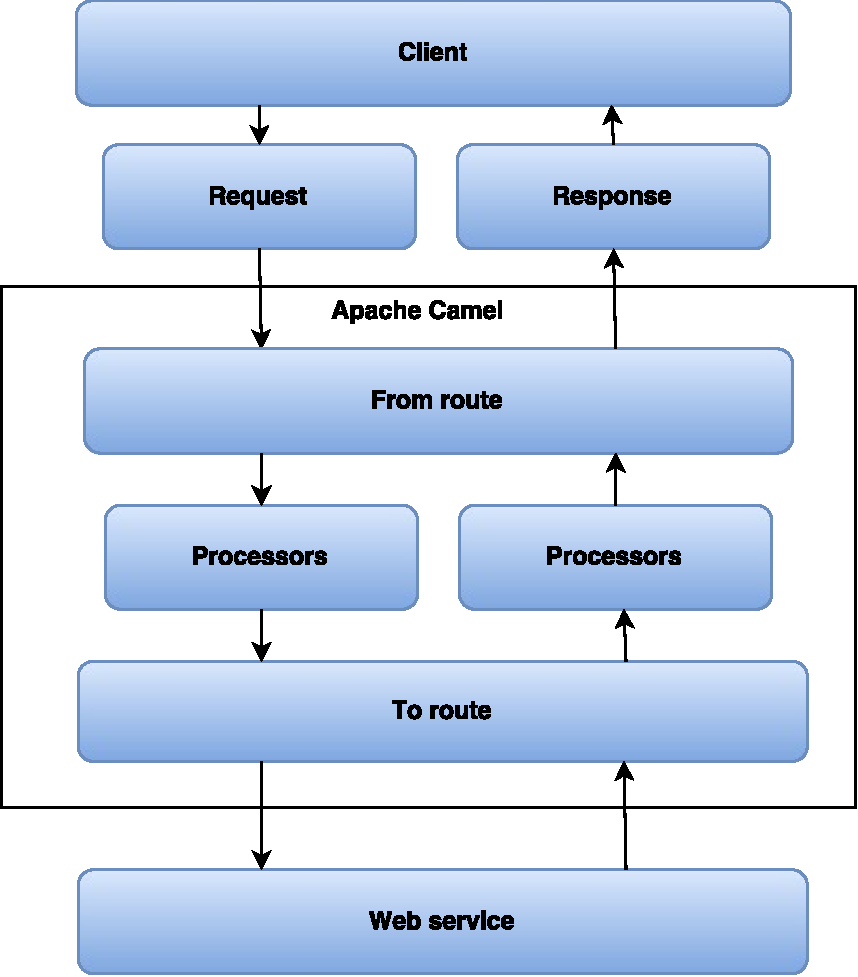
\includegraphics[scale=0.7]{images/camel_routes.pdf}
\caption{Example of a Camel route}
\label{figure:camel-route}
\end{figure}

\section{Implementation}

The proxy was implemented as a Java 1.8 application using the Apache Camel
framework. A large part of the implementation is concerned about reading user
configuration and setting up \textit{routing rules} for Apache camel. The stages
of the program are as follows:

\begin{enumerate}
    \item Reading and parsing user configuration.
    \item Initializing Camel components.
    \item Setting up routes.
    \item Running.
\end{enumerate}

\subsection{Parsing Configuration}

The first stage involves reading a user provided configuration file. Details about the configuration is explained in section X.

\subsection{Initializing Components}

Depending on which protocol the user has selected for usage as inter-proxy
communication, the respective Camel component is initiated and added to the
Camel context.

\subsubsection{HTTP Component}

We made use of the Camel component Jetty in order to consume and produce HTTP
requests. The component is based on the Jetty Web server\cite{jetty-homepage}.
It was used for two purposes: to consume \gls{http} requests from applications
and if HTTP was configured,as the selected protocol, to consume/produce HTTP
messages as part of the inter-proxy communication.

\subsubsection{AMQP Component}

Describe AMQP component.

\subsubsection{CoAP Component}

Describe CoAP component

\subsection{Routes}

A running proxy listens on two \textit{routes}. It can either receive messages
from an application, or it can receive a message from the other proxy. This
setup can be seen in \cref{figure:dil-routes}. The routing logic is different
for these two cases. We define a request origination from an outside application
as the \textit{application route}, and a request origination from another proxy
as a \textit{proxy route}. We discuss these routes, but first we need to
introduce what we have chose to call the \textit{proxy message format}.
Requirement 2 says that we need to retain all the original HTTP headers from the
original request. Consider if the proxy receives a HTTP request and forwards it
to the other protocol using AMQP. The message itself will arrive correctly, but
the original HTTP headers and method would be lost. Our approach to this was to
introduce a custom \textit{proxy message format}, which is discussed in the next
section.

\begin{figure}[h]
\centering
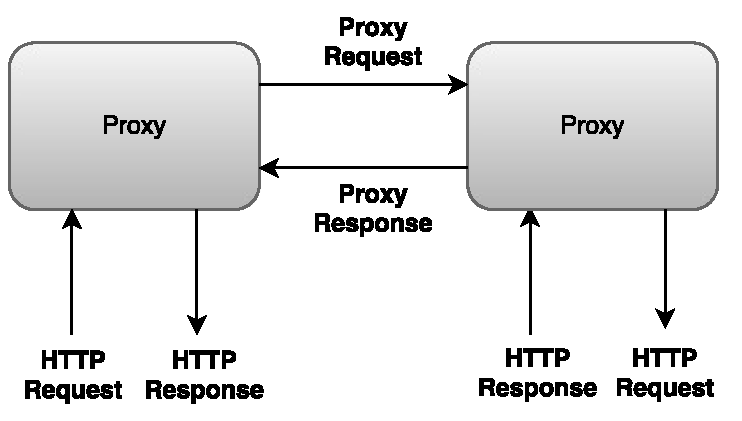
\includegraphics[scale=0.7]{images/dil_routes.pdf}
\caption{Proxy routes}
\label{figure:dil-routes}
\end{figure}

\subsection{Proxy Message Format}

The proxy message format was developed to retain HTTP headers and other
necessary information about the request. Our solution was to wrap all messages
in a JSON document and include necessary information as properties in the JSON
document. An HTTP request and response had slightly different requirements, so we
used the same format, but with different properties for a request and response.

\subsubsection{Proxy Message Request}

A proxy request message contains the following JSON fields:
\begin{description}
	\item[path] Contains the original request URL from the application. This describes the intended final destination of the original HTTP request.
	\item[method] The HTTP method of the request.
	\item[query] The query string associated with the original HTTP request.
	\item[headers] JSON object containing all the original HTTP headers of the request.
	\item[body] Contains the original payload of the message.
\end{description}

An example proxy request message is included in \cref{listing:proxy-request}.
The listing illustrates a HTTP request originating from an outside application.
It was a POST to the intended target was http://myservice.com. The payload was
an XML message.

\lstinputlisting[frame=single, language=json, firstnumber=1, caption="Example proxy request", label=listing:proxy-request]{listings/proxy_message.json}

\paragraph{}


\subsubsection{Proxy message response}

Similar to the request, but contains less fields:

\begin{description}
	\item[headers] JSON object containing the HTTP response headers.
	\item[responsecode] Contains the HTTP response code.
	\item[body] The response body of the HTTP request.
\end{description}





\subsection{Application Route}

The purpose of the application route is to consume HTTP requests from an
outside HTTP request, transform it to a proxy request message and deliver it
to the other proxy. When a response is received, return it to the application.
The route consist of the following steps:

\begin{enumerate}
	\item Defining a HTTP endpoint to consume HTTP requests from. This is read from the configuration which specifies which hostname and port to listen on.
	\item Consume HTTP request from an outside application
	\item Apply the \textit{ProxyRequestPreProcessor}. This processor converts the message into a Proxy Request Message.
	\item If compression is enabled, compress the entire message.
	\item Forward the request to the other proxy.
	\item Receive an response from the other proxy.
	\item If compression is enabled, de-compress the message.
	\item Restore the HTTP response from Proxy Response Message.
	\item Return the response to the application.
\end{enumerate}

\subsection{Proxy Route}

The purpose of the proxy route is to listen for messages from the other proxy,
de-serialize it, and deliver it to its intended receiver. When a response is
received, transform it into a Proxy Response Message and return it to the other proxy. The route consist of the following steps:

\begin{enumerate}
	\item Defining a endpoint depending on which the configured protocol.
	\item Consume requests from the other proxy.
	\item If compression is enabled, de-compress the message.
	\item Transform the message into the original HTTP request.
	\item Forward the HTTP request to its intended destination.
	\item Receive a HTTP response from the intended destination.
	\item Transform it into a Proxy Response Message.
	\item If compression is enabled, compress the message.
	\item Return the response to the other application.
\end{enumerate}

\subsection{Dealing with errors}

Discuss retransmission mechanisms

\subsection{Runtime}

In the running stage, the proxy listens on the defined routes and forward them according to the previously configured routes. All requests are logged.


\section{Functionality}

The prototype is packaged as an JAR an can be started from the command line. A path to a valid configuration file must be passed as a command line argument.


\subsection{Configuration}

\lstinputlisting[frame=single, language=json, firstnumber=1, caption="Example proxy configuration file", label=listing:proxy-config]{listings/amqp.conf}


\subsection{Proxy setup}

In order to enable the applications to tunnel all their HTTP traffic through our
proxy, we needed a way to setup a proxy without altering the applications
themselves. Fortunately, Java provide mechanisms to deal with
proxies\cite{oracle-proxy}. We configured the \gls{jvm} to get the applications
to tunnel all HTTP traffic through our proxy. This is done by setting properties
to the \gls{jvm}:


\begin{lstlisting}[frame=single, caption="Setting a proxy on the \gls{jvm}", label=test]
java -Dhttp.proxyHost=localhost \
-Dhttp.proxyPort=3001 \
-Dhttp.nonProxyHosts= \
-jar target/client.jar
\end{lstlisting}

In \cref{test} the application \textbf{client.jar} is started and all HTTP
traffic will go through the proxy server at localhost on port 3001.


\section{CoAP component}

Elaborate about the custom CoAP component here.

\section{Summary}

In this chapter we presented the design and implementation details of the proxy
